\documentclass[letterpaper,twoside]{article}

\usepackage[authoryear]{natbib}
\usepackage{times} 
\usepackage{amsmath,amsfonts}
\usepackage{graphicx}
\usepackage{indentfirst}
\usepackage{color}
\usepackage{url}
\usepackage[paper=letterpaper]{geometry}
\usepackage{fontspec}
\setmainfont[Mapping=text-tex]{Calibri}

% revise margins
\setlength{\headheight}{0.25in}
\setlength{\headsep}{-0.25in}
\setlength{\topmargin}{0.0in}
\setlength{\textheight}{9in}
\setlength{\footskip}{0.5in}
\setlength{\oddsidemargin}{-0.25in}
\setlength{\evensidemargin}{-0.25in}
\setlength{\textwidth}{7.0in}
\setlength{\rightskip}{0pt plus 1fil} % makes ragged right

% headings
\usepackage{fancyhdr}
\pagestyle{fancy}
\fancyfoot{}
\fancyfoot[C]{K. W. Broman \emph{et al.}}
\fancyfoot[RO, LE]{\textbf{\thepage\ SI}}
\fancyhead{}
\renewcommand{\headrulewidth}{0pt}
\renewcommand{\footrulewidth}{0pt}

\begin{document}

\vspace*{8mm}
\begin{center}

\textbf{\Large Mapping quantitative trait loci %\\[18pt] 
onto a phylogenetic tree}
 
 
\bigskip \bigskip \bigskip \bigskip 
 
\textbf{\Large SUPPLEMENT}

\bigskip \bigskip
\bigskip \bigskip
 
 
{\large Karl W. Broman$^{*}$, Sungjin Kim$^{\dagger}$, \'Saunak
  Sen$^\ddagger$,\\[6pt]
C\'ecile An\'e$^{\dagger,\S}$, Bret A. Payseur$^{**}$}

\bigskip \bigskip

$^*$Department of Biostatistics and Medical Informatics,
$^\dagger$Department of Statistics, $^{\S}$Department of Botany, and $^{**}$Laboratory of
Genetics, University of Wisconsin--Madison, Madison, Wisconsin
53706; $^\ddagger$Department of Epidemiology and Biostatistics, University
of California, San Francisco, San Francisco, California 94107
\end{center}


%\vfill
%
%\hfill 
%{\footnotesize 24 February 2012}

\newpage

{\centering
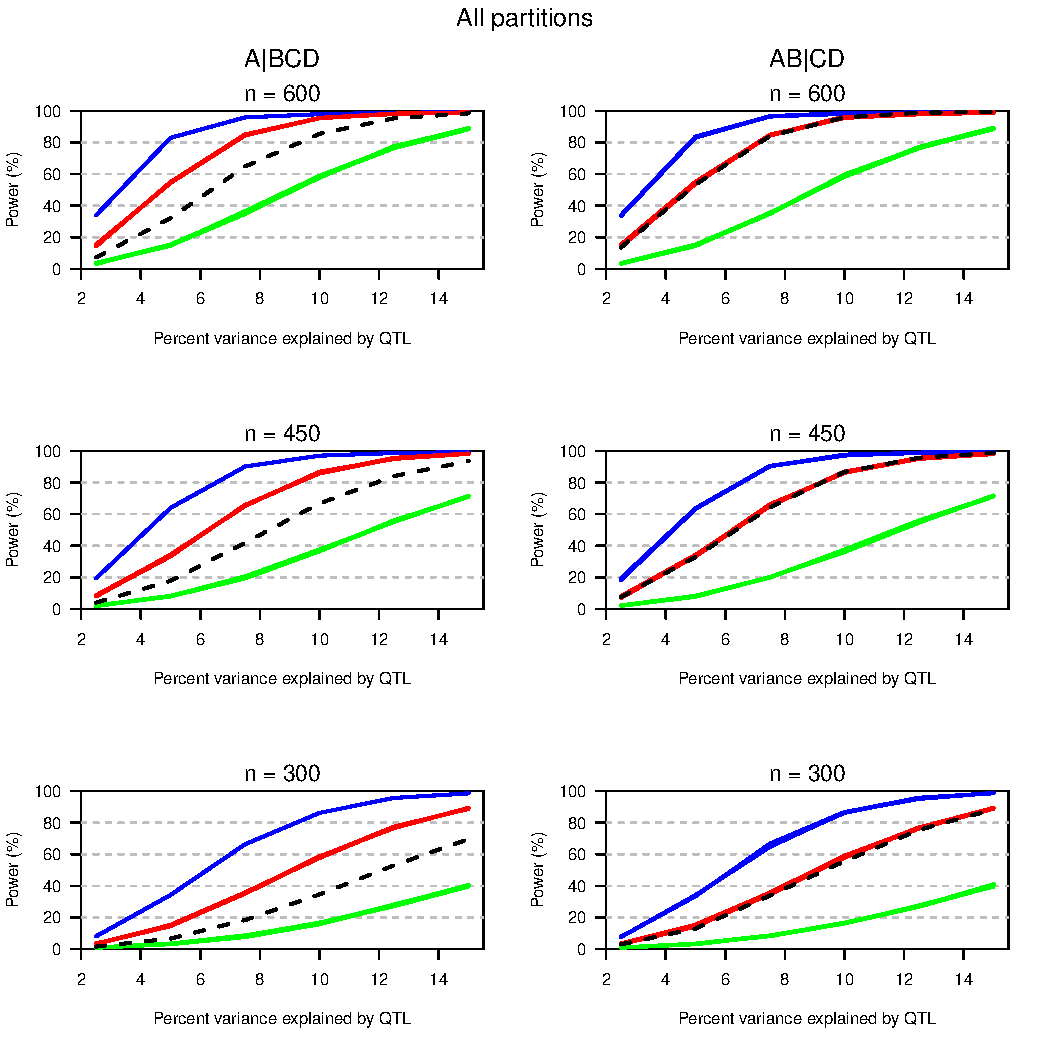
\includegraphics{SuppFigs/power_allpart.pdf}}

\bigskip \noindent
Figure S1: Estimated power in the case of four taxa with a total
  sample size of either 300 (bottom panels) 450 (middle panels) or 600
  (top panels), as a function of the percent phenotypic variance
  explained by the QTL.  The black dashed curves correspond to the use
  of all six possible crosses.  The other curves are for the various
  choices of a minimal set of three crosses, with the curves in blue,
  red and green corresponding to cases in which 3, 2 and 1 of the
  crosses are segregating the QTL, respectively.  The results are
  based on 10,000 simulation replicates, with analyses considering all
  possible partitions of the taxa.

\newpage


{\centering
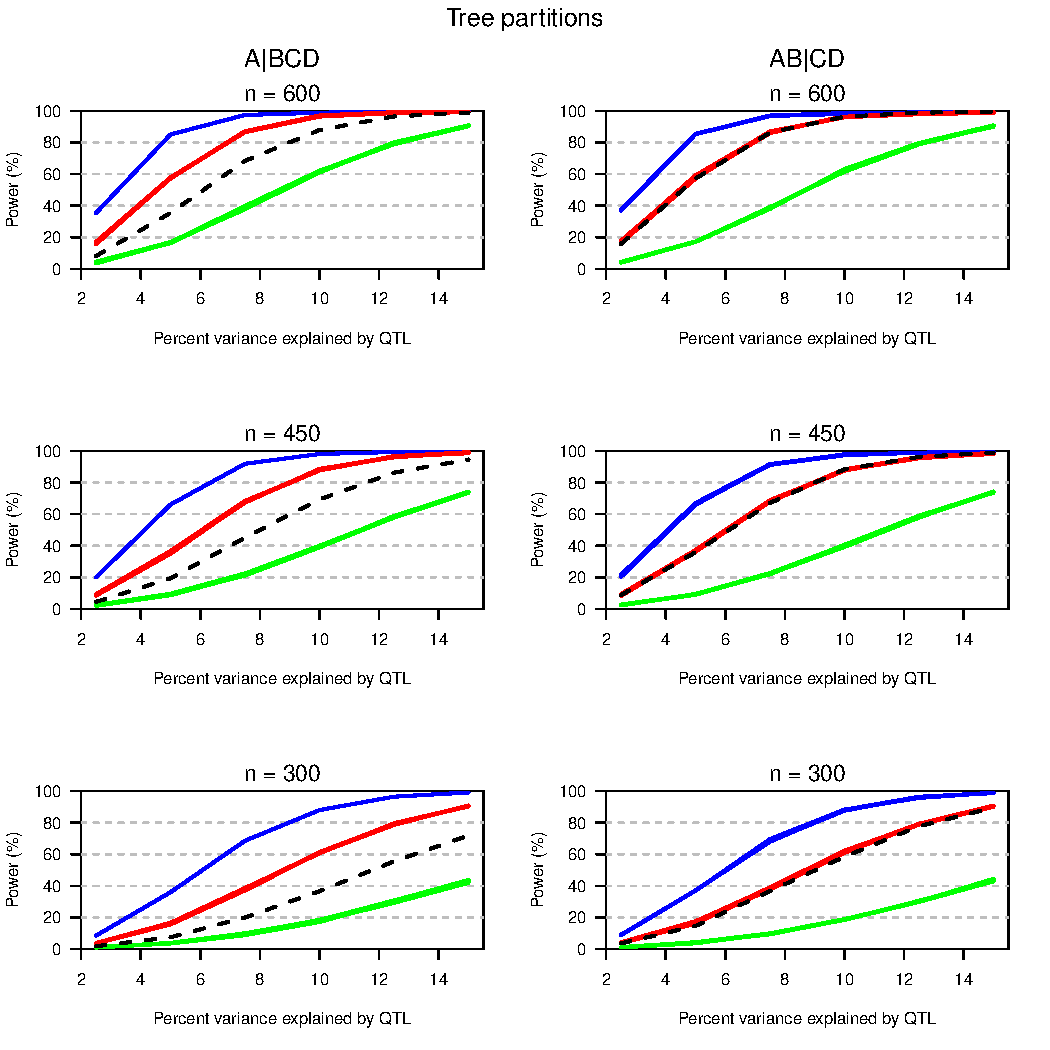
\includegraphics{SuppFigs/power_treepart.pdf}}

\bigskip \noindent
Figure S2: Estimated power in the case of four taxa related as in
  Figure~1, and with a total sample size of either 300 (bottom panels)
  450 (middle panels) or 600 (top panels), as a function of the
  percent phenotypic variance explained by the QTL.  The black dashed
  curves correspond to the use of all six possible crosses.  The other
  curves are for the various choices of a minimal set of three
  crosses, with the curves in blue, red and green corresponding to
  cases in which 3, 2 and 1 of the crosses are segregating the QTL,
  respectively.  The results are based on 10,000 simulation
  replicates, with analyses considering only the four possible
  partitions induced by the tree.

\newpage

{\centering
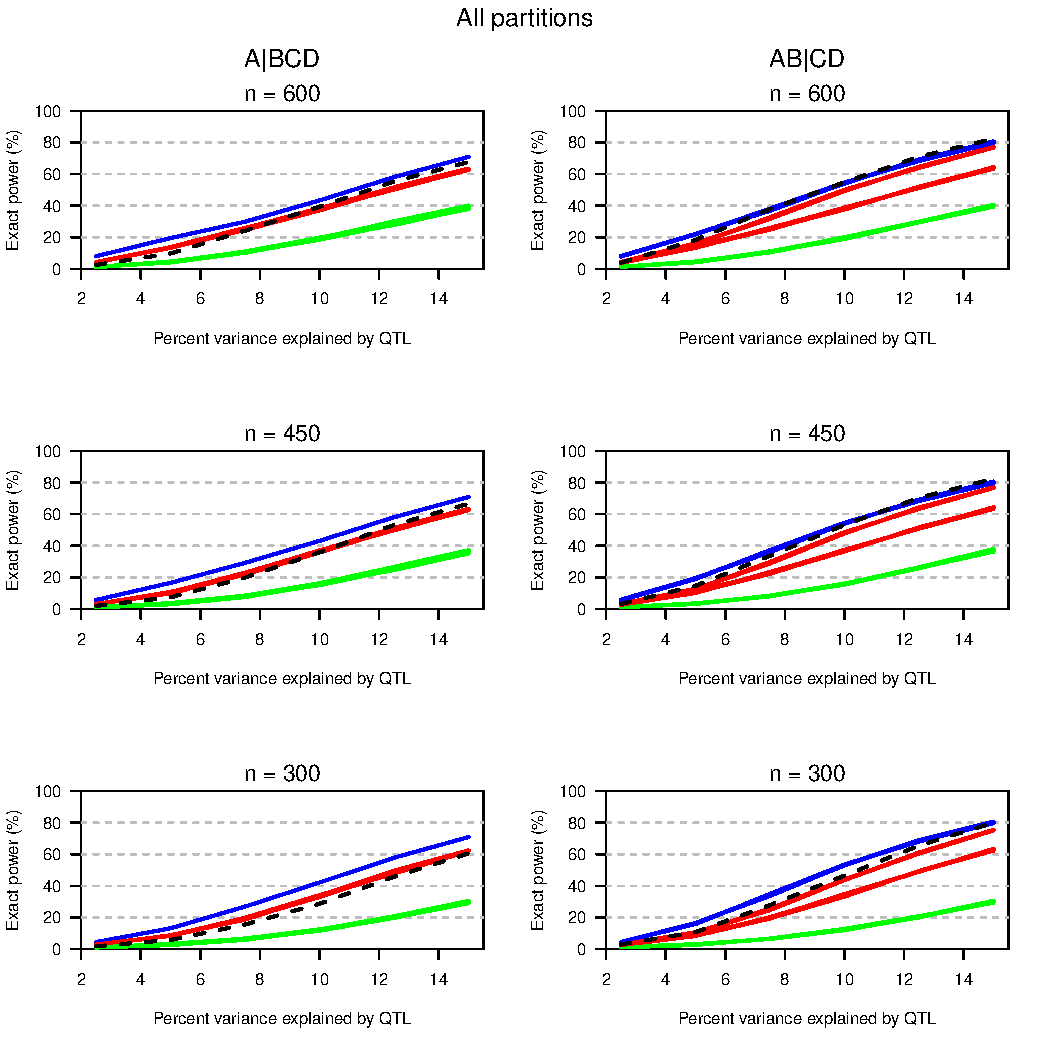
\includegraphics{SuppFigs/expower_allpart.pdf}}

\bigskip \noindent
Figure S3: Estimated ``exact'' power (the chance that a QTL is detected and the
credible set of partitions contains only the true partion) in the case of four taxa with a total
  sample size of either 300 (bottom panels) 450 (middle panels) or 600
  (top panels), as a function of the percent phenotypic variance
  explained by the QTL.  The black dashed curves correspond to the use
  of all six possible crosses.  The other curves are for the various
  choices of a minimal set of three crosses, with the curves in blue,
  red and green corresponding to cases in which 3, 2 and 1 of the
  crosses are segregating the QTL, respectively.  The results are
  based on 10,000 simulation replicates, with analyses considering all
  possible partitions of the taxa.

\newpage

{\centering
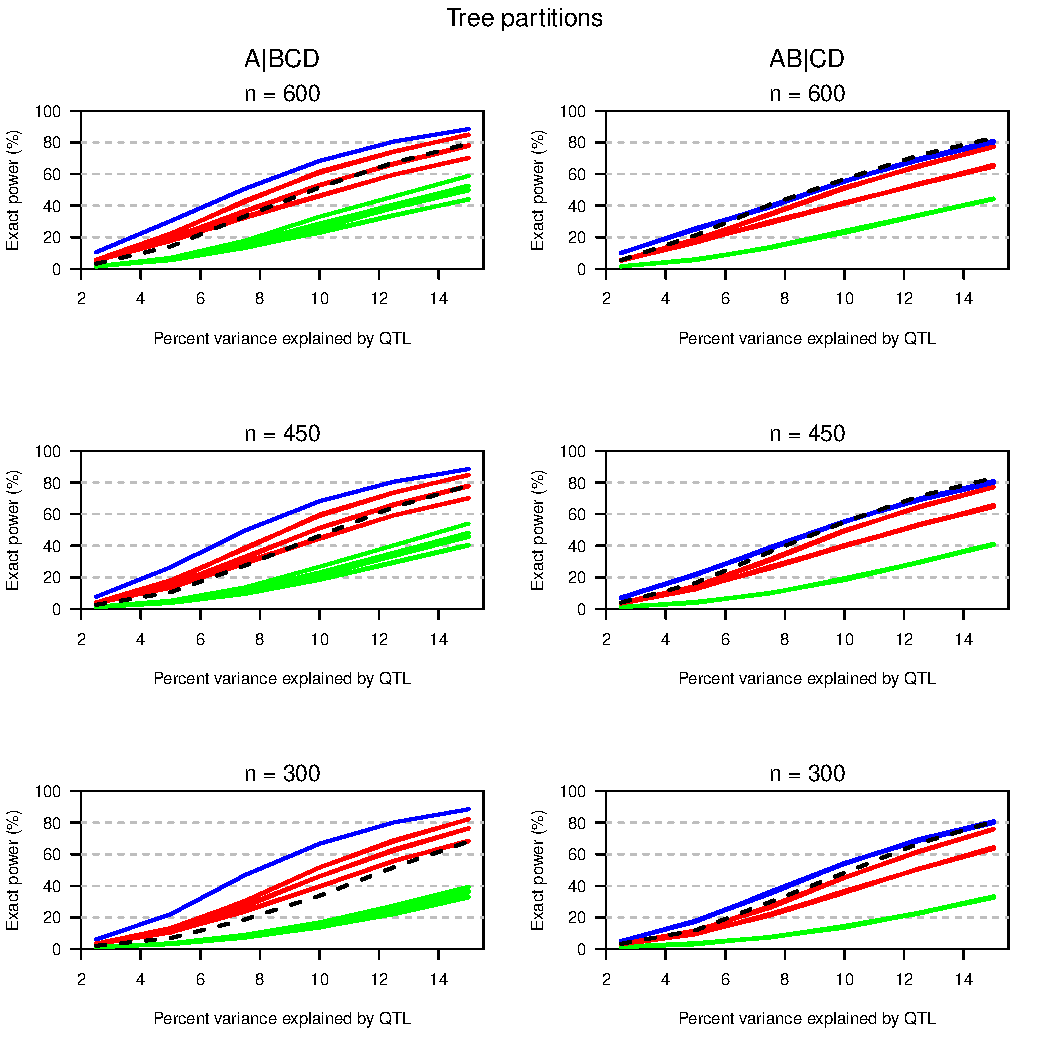
\includegraphics{SuppFigs/expower_treepart.pdf}}

\bigskip \noindent
Figure S4: Estimated ``exact'' power (the chance that a QTL is detected and the
credible set of partitions contains only the true partion) in the case of four taxa related as in
  Figure~1, and with a total sample size of either 300 (bottom panels)
  450 (middle panels) or 600 (top panels), as a function of the
  percent phenotypic variance explained by the QTL.  The black dashed
  curves correspond to the use of all six possible crosses.  The other
  curves are for the various choices of a minimal set of three
  crosses, with the curves in blue, red and green corresponding to
  cases in which 3, 2 and 1 of the crosses are segregating the QTL,
  respectively.  The results are based on 10,000 simulation
  replicates, with analyses considering only the four possible
  partitions induced by the tree.

\newpage

{\centering
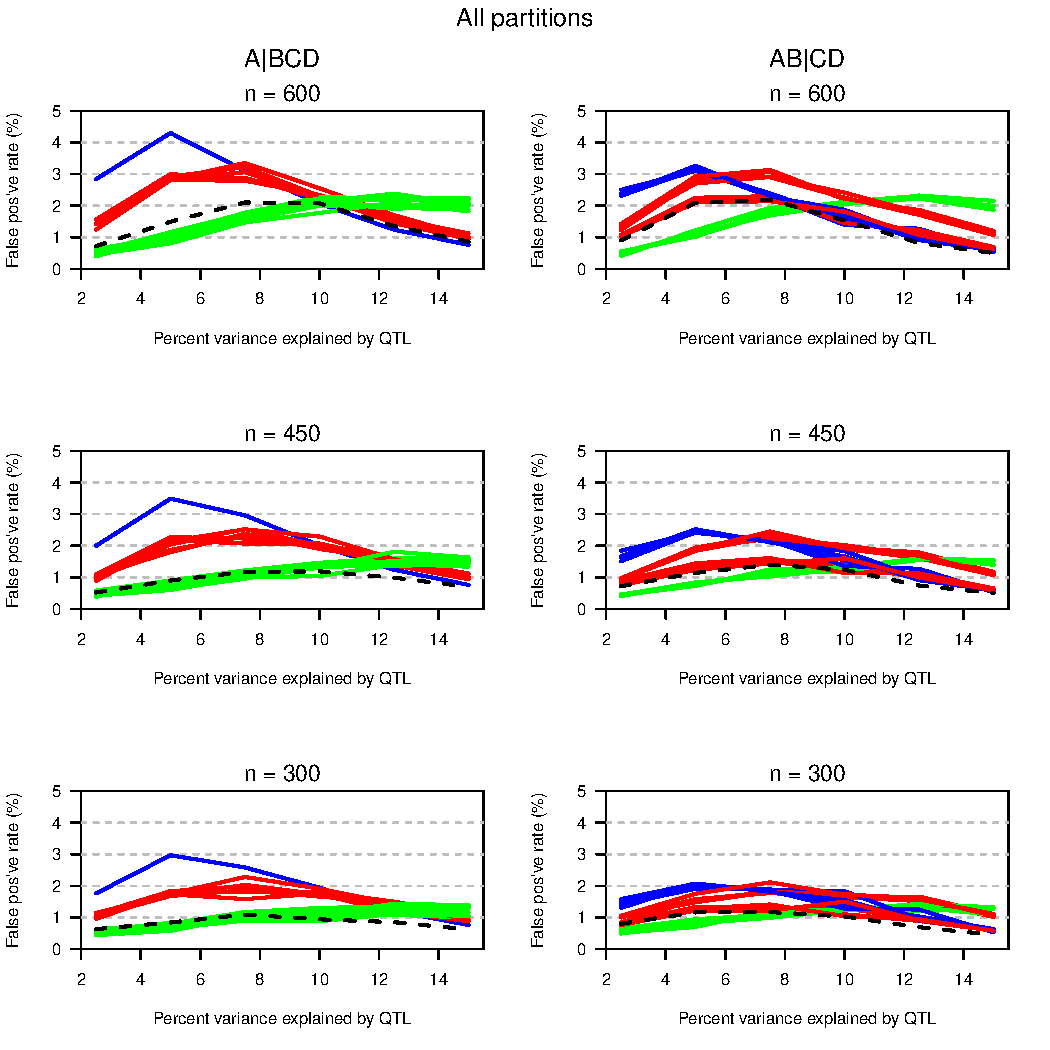
\includegraphics{SuppFigs/fp_allpart.pdf}}

\bigskip \noindent
Figure S5: Estimated false positive rate in the case of four taxa with a total
  sample size of either 300 (bottom panels) 450 (middle panels) or 600
  (top panels), as a function of the percent phenotypic variance
  explained by the QTL.  The black dashed curves correspond to the use
  of all six possible crosses.  The other curves are for the various
  choices of a minimal set of three crosses, with the curves in blue,
  red and green corresponding to cases in which 3, 2 and 1 of the
  crosses are segregating the QTL, respectively.  The results are
  based on 10,000 simulation replicates, with analyses considering all
  possible partitions of the taxa.

\newpage

{\centering
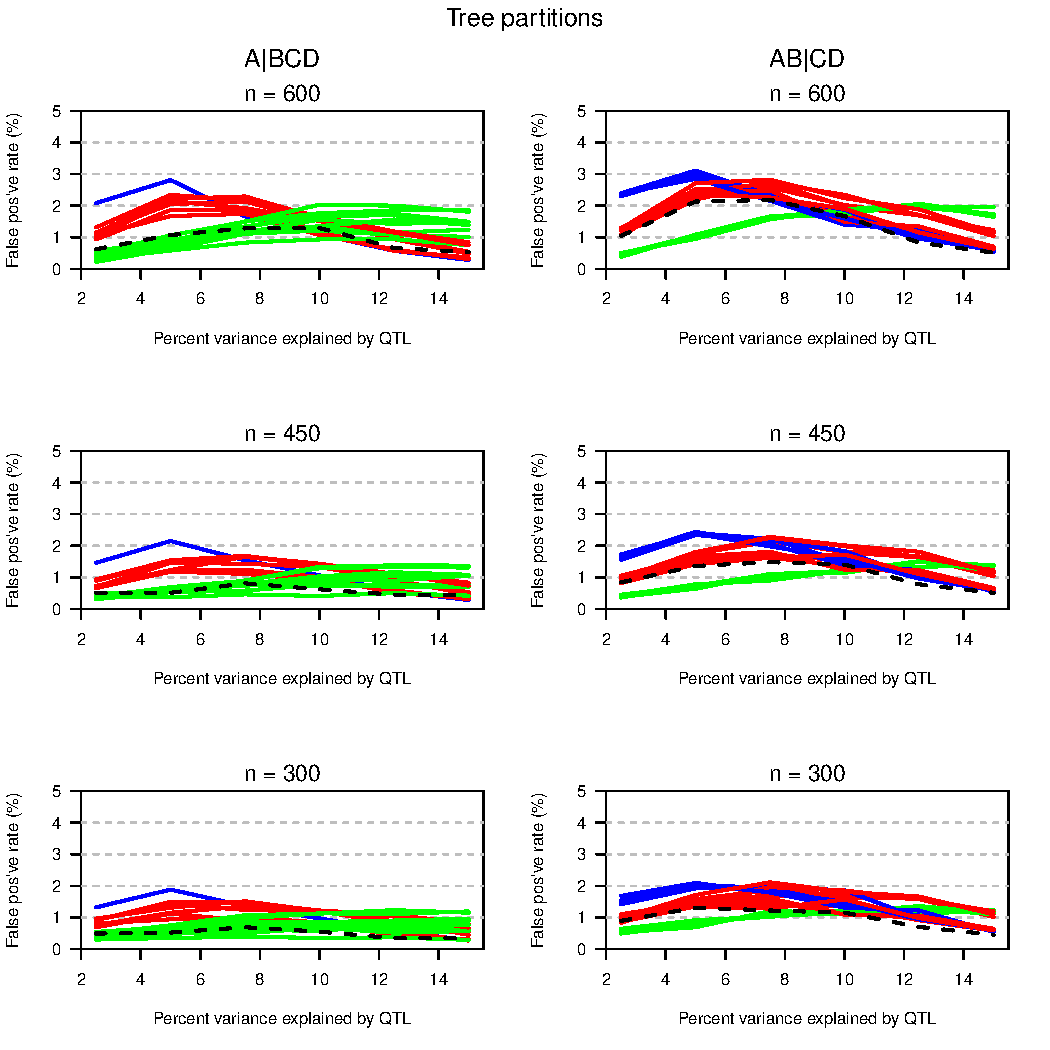
\includegraphics{SuppFigs/fp_treepart.pdf}}

\bigskip \noindent
Figure S6: Estimated false positive rate in the case of four taxa related as in
  Figure~1, and with a total sample size of either 300 (bottom panels)
  450 (middle panels) or 600 (top panels), as a function of the
  percent phenotypic variance explained by the QTL.  The black dashed
  curves correspond to the use of all six possible crosses.  The other
  curves are for the various choices of a minimal set of three
  crosses, with the curves in blue, red and green corresponding to
  cases in which 3, 2 and 1 of the crosses are segregating the QTL,
  respectively.  The results are based on 10,000 simulation
  replicates, with analyses considering only the four possible
  partitions induced by the tree.

\newpage

{\centering
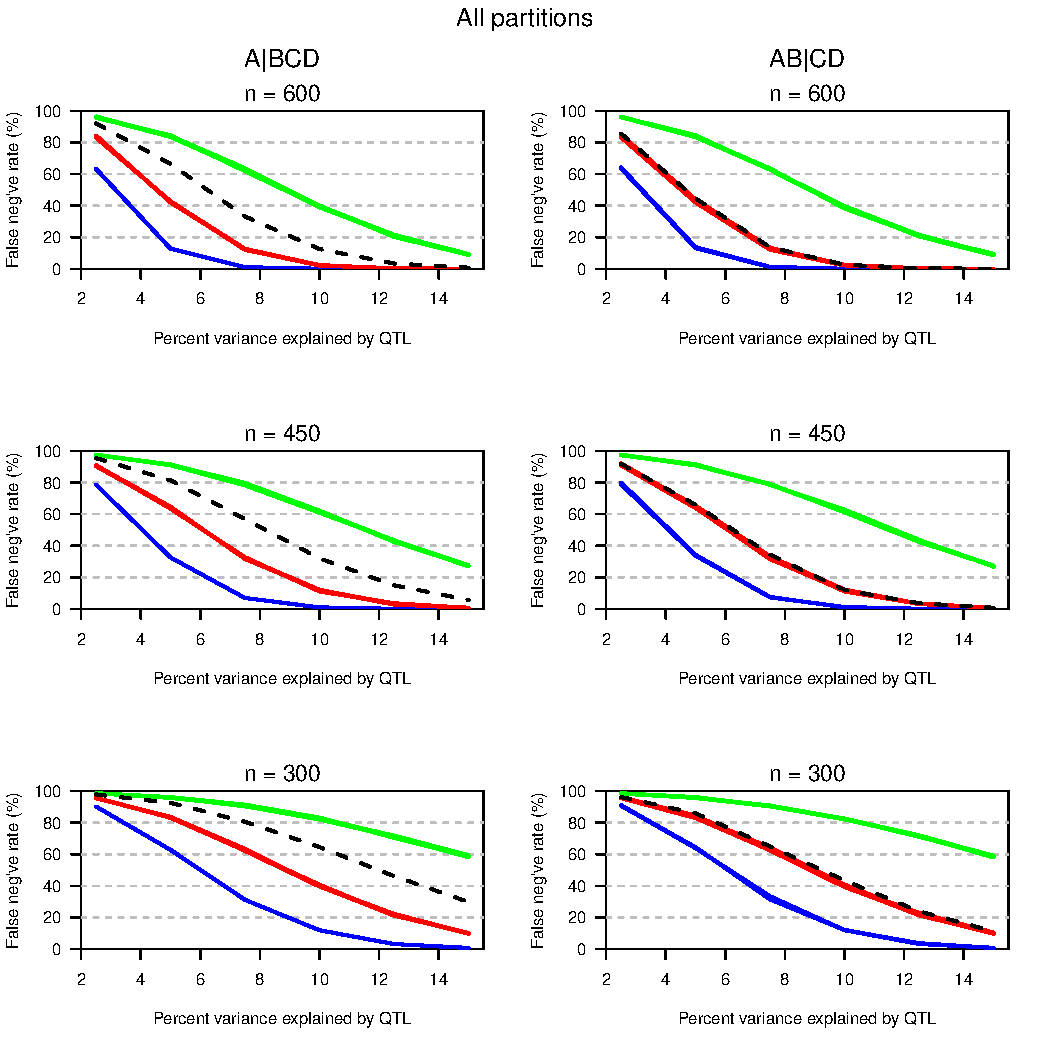
\includegraphics{SuppFigs/ns_allpart.pdf}}

\bigskip \noindent
Figure S7: Estimated false negative rate in the case of four taxa with a total
  sample size of either 300 (bottom panels) 450 (middle panels) or 600
  (top panels), as a function of the percent phenotypic variance
  explained by the QTL.  The black dashed curves correspond to the use
  of all six possible crosses.  The other curves are for the various
  choices of a minimal set of three crosses, with the curves in blue,
  red and green corresponding to cases in which 3, 2 and 1 of the
  crosses are segregating the QTL, respectively.  The results are
  based on 10,000 simulation replicates, with analyses considering all
  possible partitions of the taxa.

\newpage

{\centering
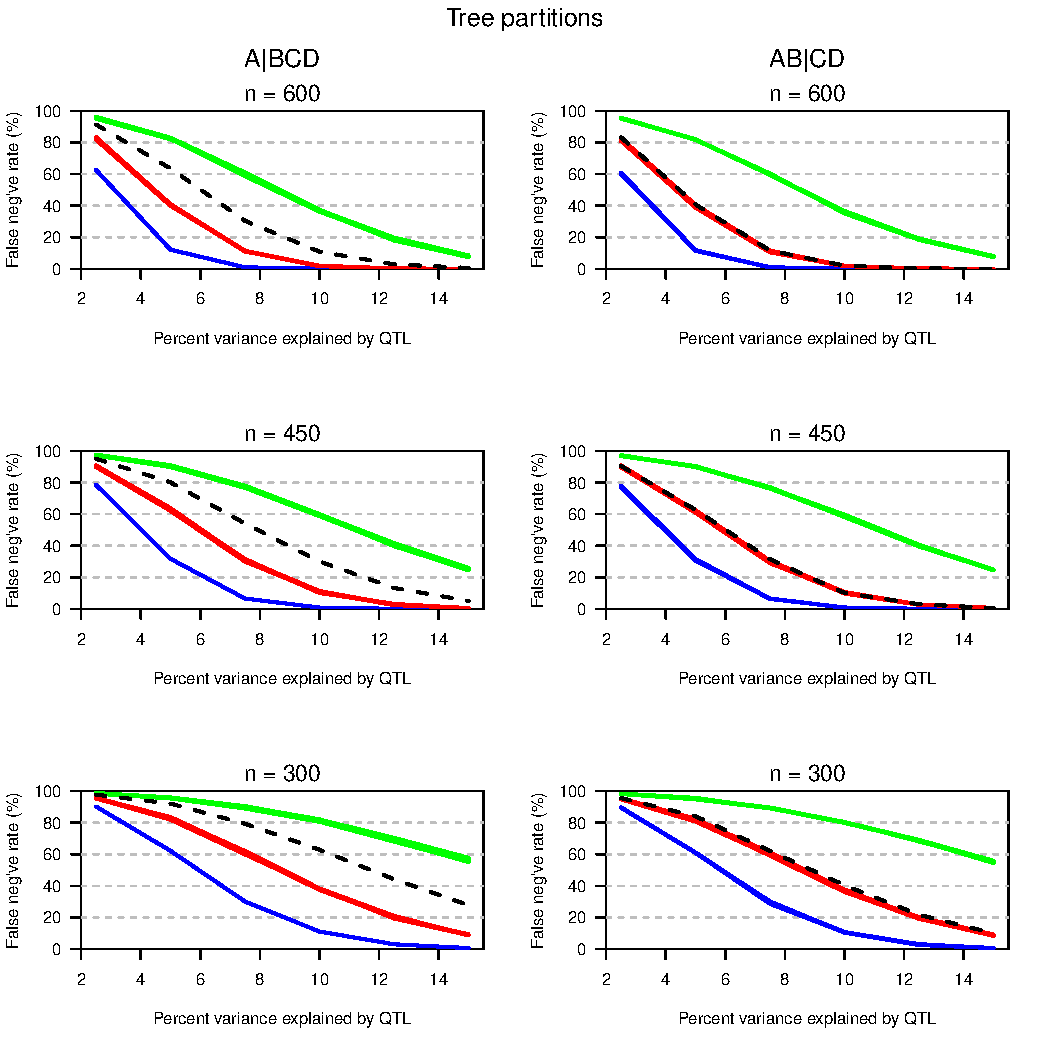
\includegraphics{SuppFigs/ns_treepart.pdf}}

\bigskip \noindent
Figure S8: Estimated false negative rate in the case of four taxa related as in
  Figure~1, and with a total sample size of either 300 (bottom panels)
  450 (middle panels) or 600 (top panels), as a function of the
  percent phenotypic variance explained by the QTL.  The black dashed
  curves correspond to the use of all six possible crosses.  The other
  curves are for the various choices of a minimal set of three
  crosses, with the curves in blue, red and green corresponding to
  cases in which 3, 2 and 1 of the crosses are segregating the QTL,
  respectively.  The results are based on 10,000 simulation
  replicates, with analyses considering only the four possible
  partitions induced by the tree.

\newpage

{\centering
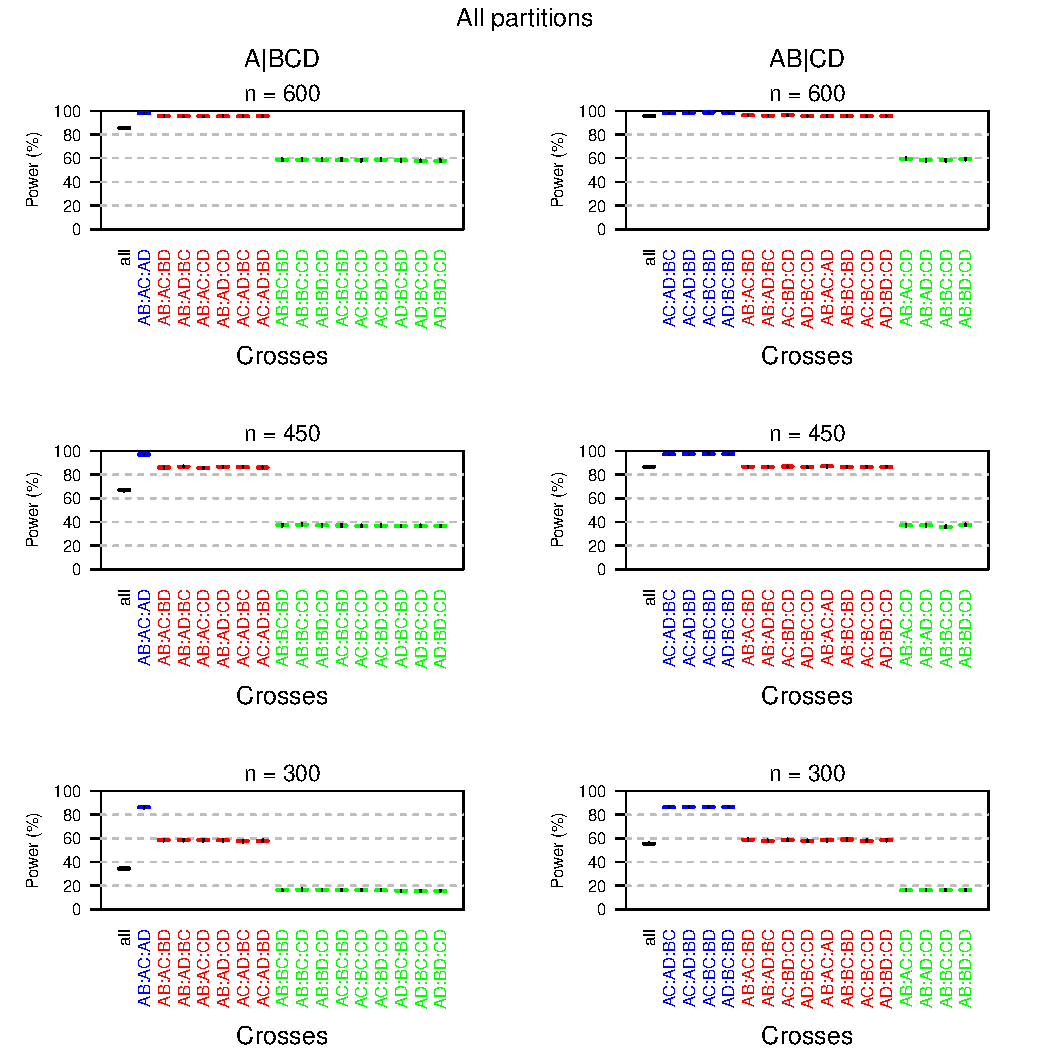
\includegraphics{SuppFigs/detailedpower_allpart.pdf}}

\bigskip \noindent
Figure S9: Detailed results on the estimated power
  for individual choices of crosses, in the case of four taxa
  with a total sample size of either 300 (bottom panels)
  450 (middle panels) or 600 (top panels),
  and with the QTL being responsible
  for 10\% of the phenotypic variance in crosses in which it is
  segregating. Blue, red and green correspond to cases in which 3, 2,
  and 1 of the crosses are segregating the QTL, respectively.  The
  results are based on 10,000 simulation replicates, with analyses
  considering all possible partitions of the taxa.  The black vertical
  line segments indicate 95\% confidence
  intervals.

\newpage

{\centering
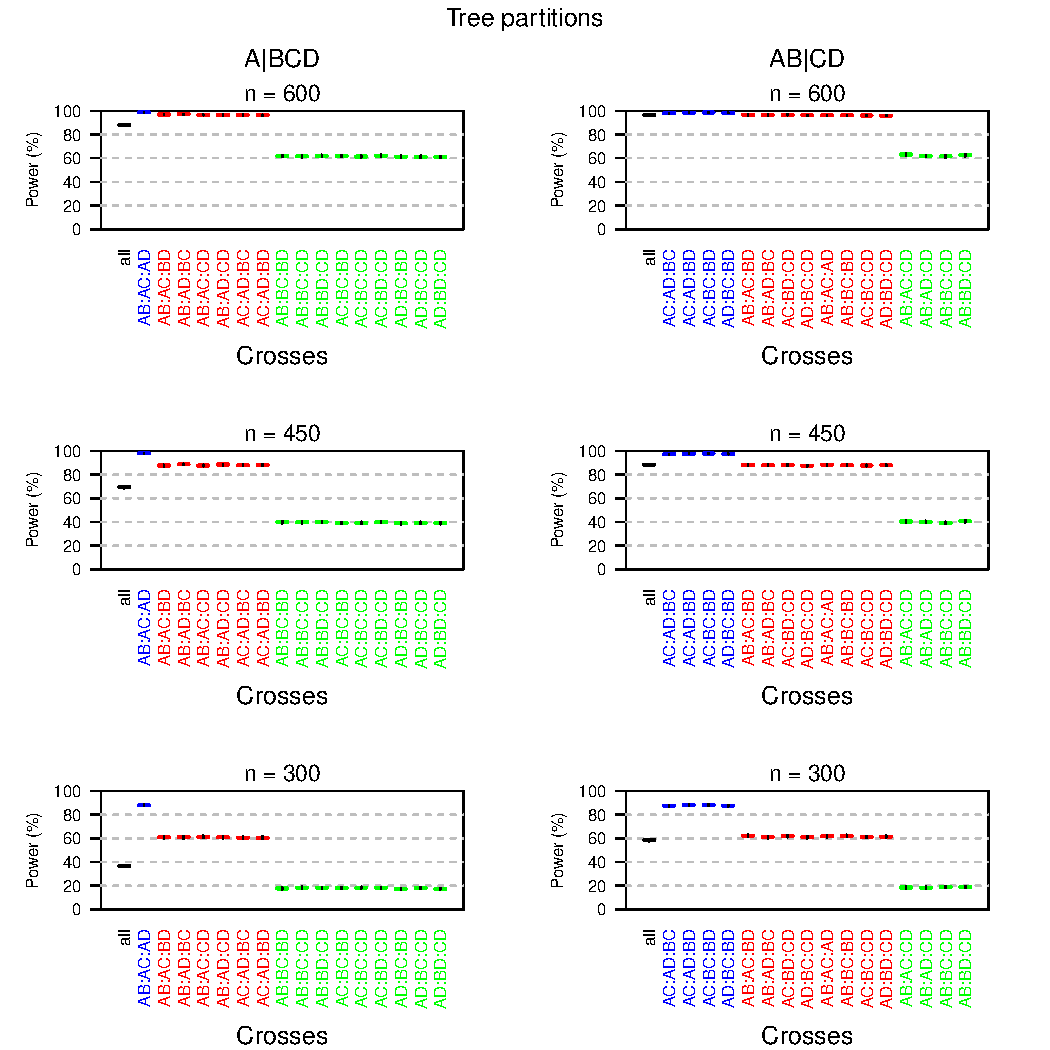
\includegraphics{SuppFigs/detailedpower_treepart.pdf}}

\bigskip \noindent
Figure S10: Detailed results on the estimated power for individual
  choices of crosses, in the case of four taxa related as in Figure~1,
  with a total sample size of either 300 (bottom panels) 450 (middle
  panels) or 600 (top panels), and with the QTL being responsible
  for 10\% of the phenotypic variance in crosses in which it is
  segregating. Blue, red and green correspond to cases in which 3, 2,
  and 1 of the crosses are segregating the QTL, respectively.  The
  results are based on 10,000 simulation replicates, with analyses
  considering only the four possible partitions induced by the tree.
  The black vertical line segments indicate 95\% confidence intervals.

\newpage

{\centering
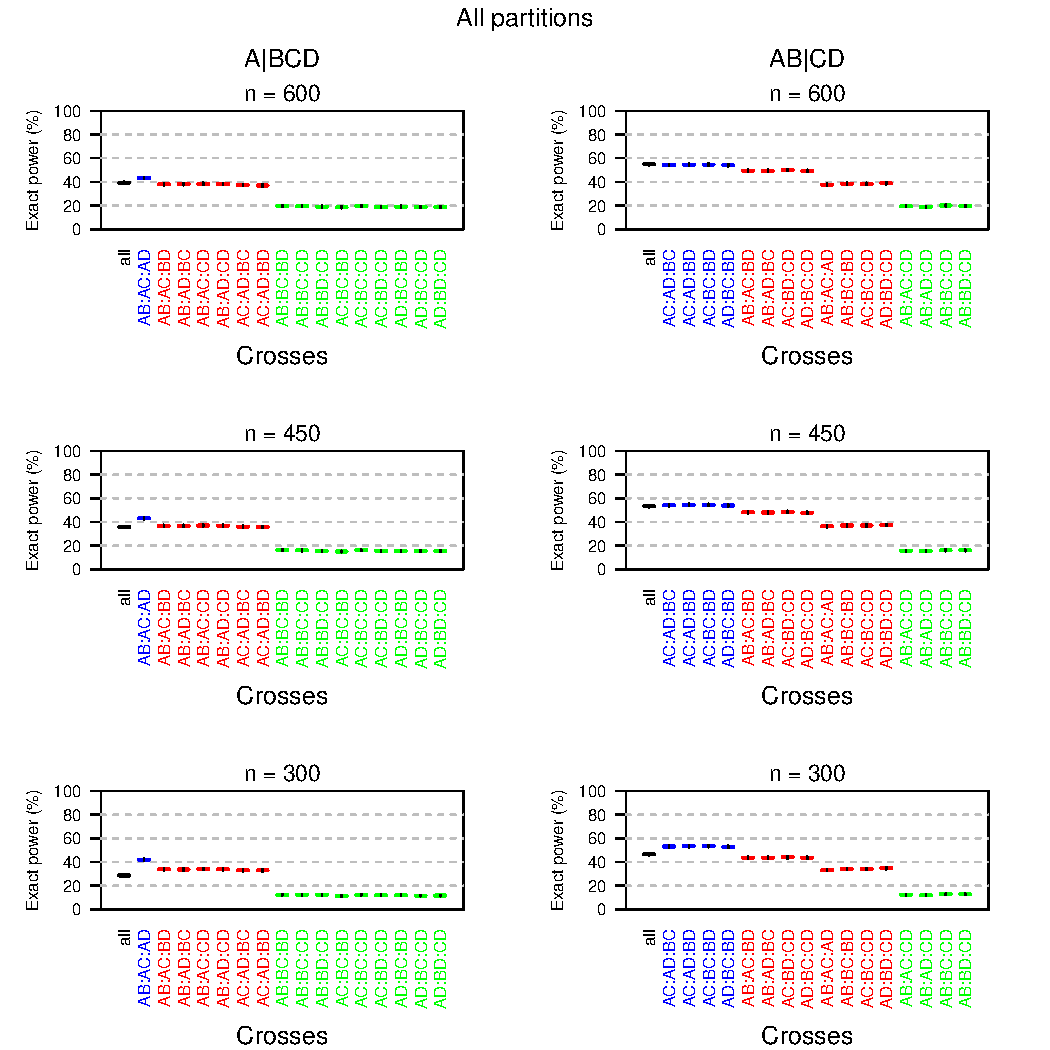
\includegraphics{SuppFigs/detailedexpower_allpart.pdf}}

\bigskip \noindent
Figure S11: Detailed results on the estimated ``exact'' power
  (the chance that a QTL is detected and the
credible set of partitions contains only the true partion) for individual choices of crosses, in the case of four taxa
  with a total sample size of either 300 (bottom panels)
  450 (middle panels) or 600 (top panels),
  and with the QTL being responsible
  for 10\% of the phenotypic variance in crosses in which it is
  segregating. Blue, red and green correspond to cases in which 3, 2,
  and 1 of the crosses are segregating the QTL, respectively.  The
  results are based on 10,000 simulation replicates, with analyses
  considering all possible partitions of the taxa.  The black vertical
  line segments indicate 95\% confidence
  intervals.

\newpage

{\centering
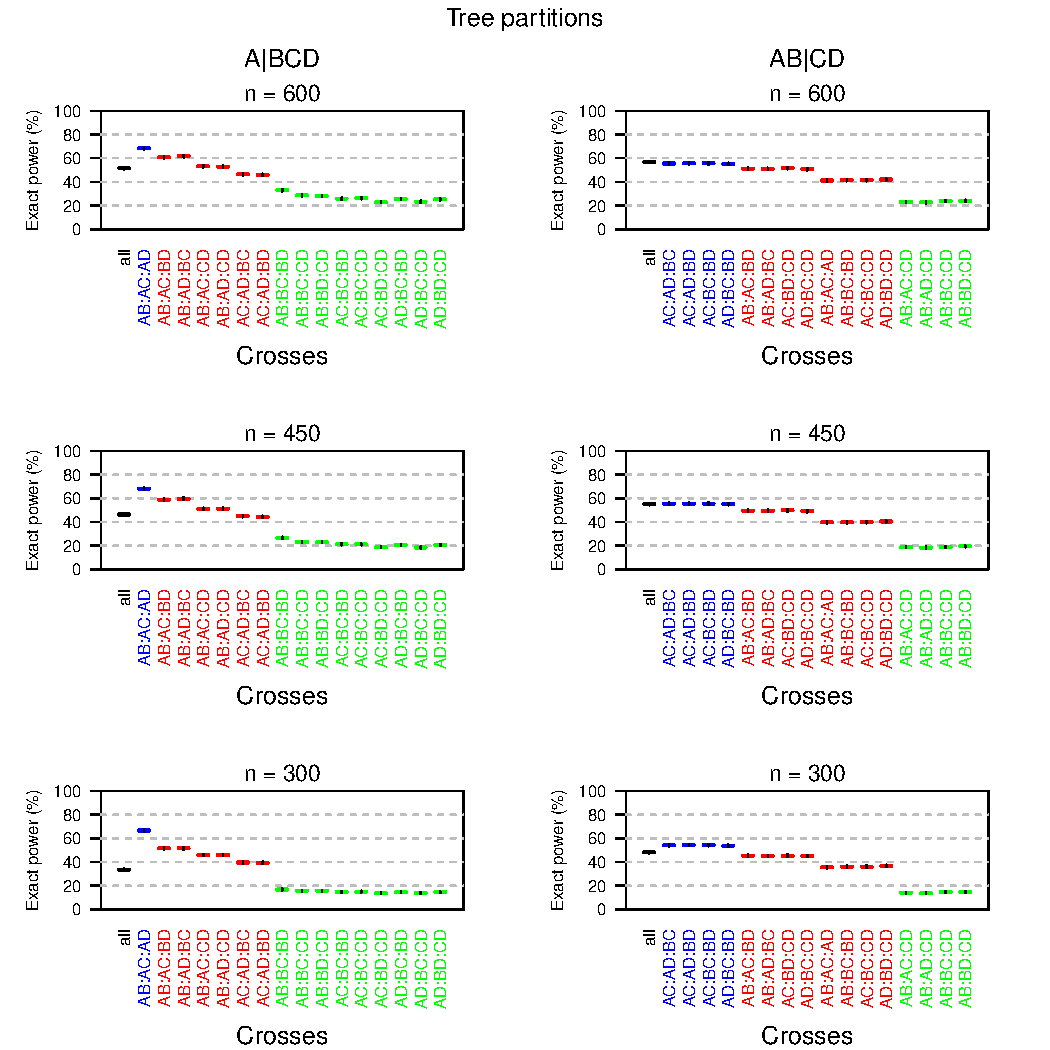
\includegraphics{SuppFigs/detailedexpower_treepart.pdf}}

\bigskip \noindent
Figure S12: Detailed results on the estimated ``exact'' power (the chance that a QTL is detected and the
credible set of partitions contains only the true partion) for individual
  choices of crosses, in the case of four taxa related as in Figure~1,
  with a total sample size of either 300 (bottom panels) 450 (middle
  panels) or 600 (top panels), and with the QTL being responsible
  for 10\% of the phenotypic variance in crosses in which it is
  segregating. Blue, red and green correspond to cases in which 3, 2,
  and 1 of the crosses are segregating the QTL, respectively.  The
  results are based on 10,000 simulation replicates, with analyses
  considering only the four possible partitions induced by the tree.
  The black vertical line segments indicate 95\% confidence intervals.

\newpage

{\centering
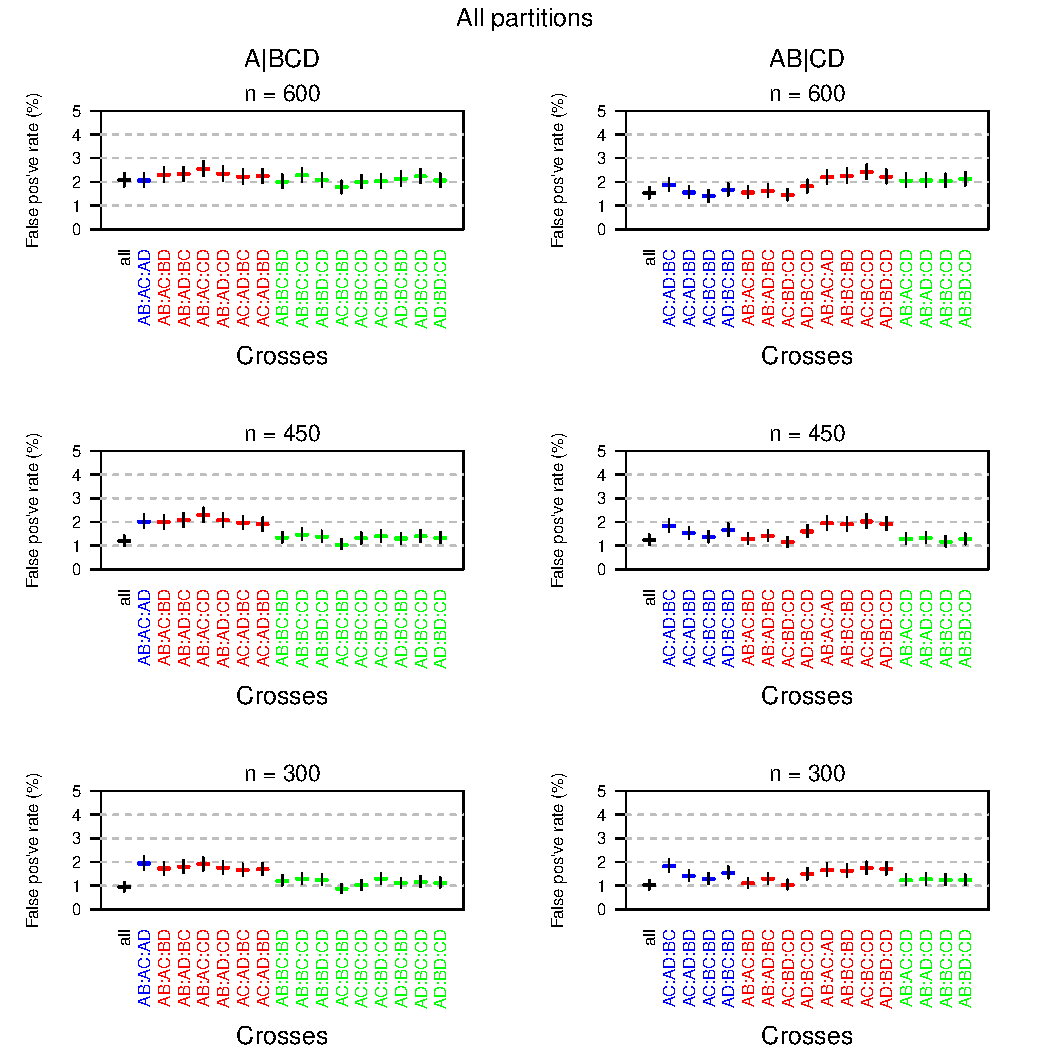
\includegraphics{SuppFigs/detailedfp_allpart.pdf}}

\bigskip \noindent
Figure S13: Detailed results on the estimated false positive rate
  for individual choices of crosses, in the case of four taxa
  with a total sample size of either 300 (bottom panels)
  450 (middle panels) or 600 (top panels),
  and with the QTL being responsible
  for 10\% of the phenotypic variance in crosses in which it is
  segregating. Blue, red and green correspond to cases in which 3, 2,
  and 1 of the crosses are segregating the QTL, respectively.  The
  results are based on 10,000 simulation replicates, with analyses
  considering all possible partitions of the taxa.  The black vertical
  line segments indicate 95\% confidence
  intervals.

\newpage

{\centering
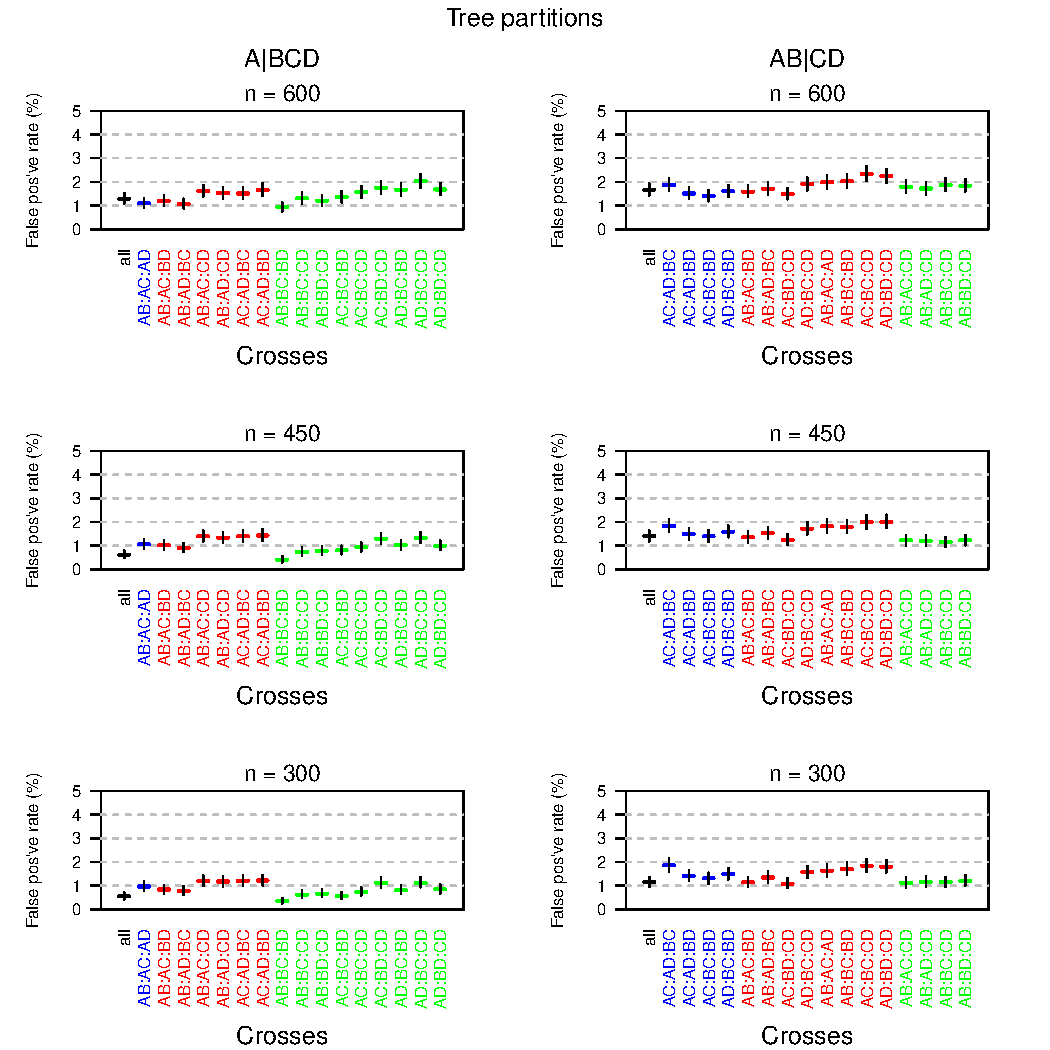
\includegraphics{SuppFigs/detailedfp_treepart.pdf}}

\bigskip \noindent
Figure S14: Detailed results on the estimated false positive rate for individual
  choices of crosses, in the case of four taxa related as in Figure~1,
  with a total sample size of either 300 (bottom panels) 450 (middle
  panels) or 600 (top panels), and with the QTL being responsible
  for 10\% of the phenotypic variance in crosses in which it is
  segregating. Blue, red and green correspond to cases in which 3, 2,
  and 1 of the crosses are segregating the QTL, respectively.  The
  results are based on 10,000 simulation replicates, with analyses
  considering only the four possible partitions induced by the tree.
  The black vertical line segments indicate 95\% confidence intervals.

\newpage

{\centering
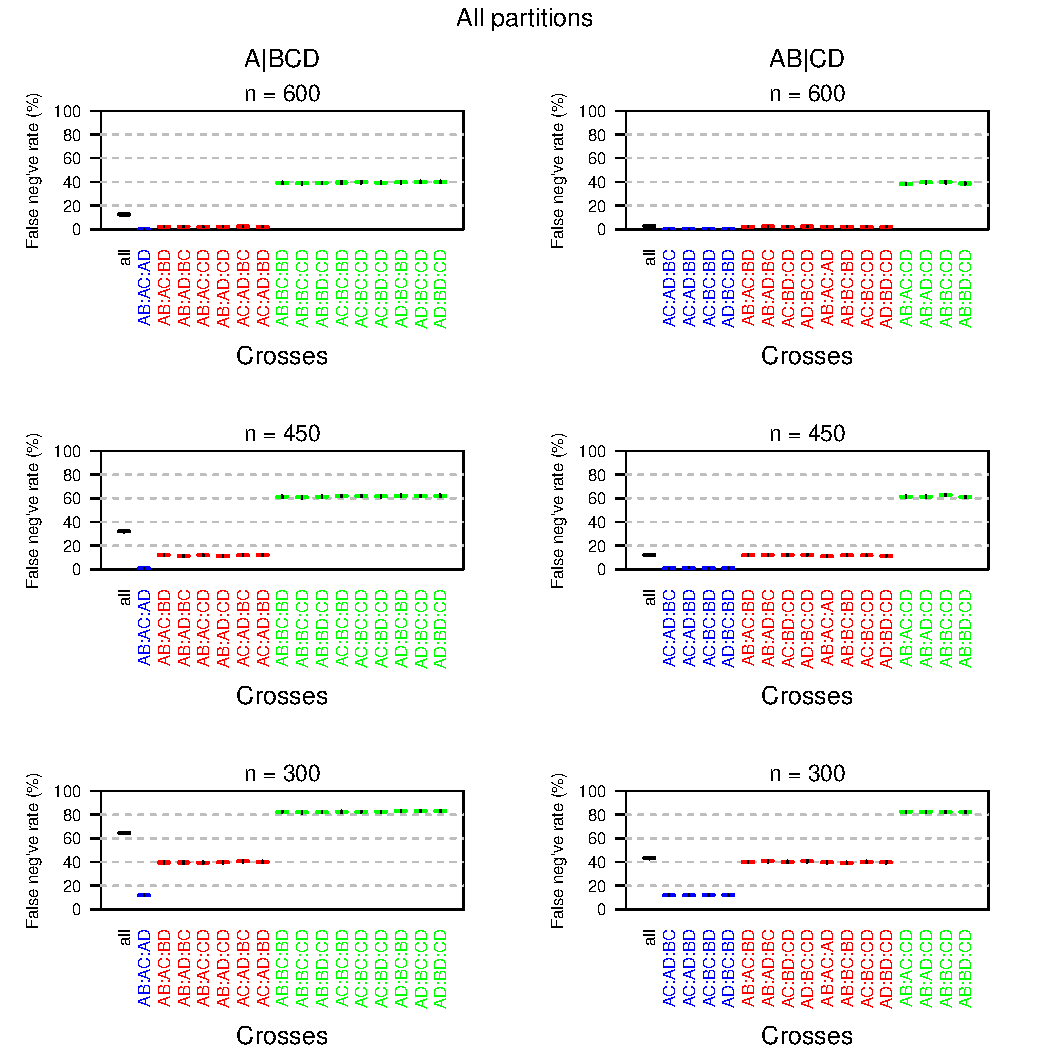
\includegraphics{SuppFigs/detailedns_allpart.pdf}}

\bigskip \noindent
Figure S15: Detailed results on the estimated false negative rate
  for individual choices of crosses, in the case of four taxa
  with a total sample size of either 300 (bottom panels)
  450 (middle panels) or 600 (top panels),
  and with the QTL being responsible
  for 10\% of the phenotypic variance in crosses in which it is
  segregating. Blue, red and green correspond to cases in which 3, 2,
  and 1 of the crosses are segregating the QTL, respectively.  The
  results are based on 10,000 simulation replicates, with analyses
  considering all possible partitions of the taxa.  The black vertical
  line segments indicate 95\% confidence
  intervals.

\newpage

{\centering
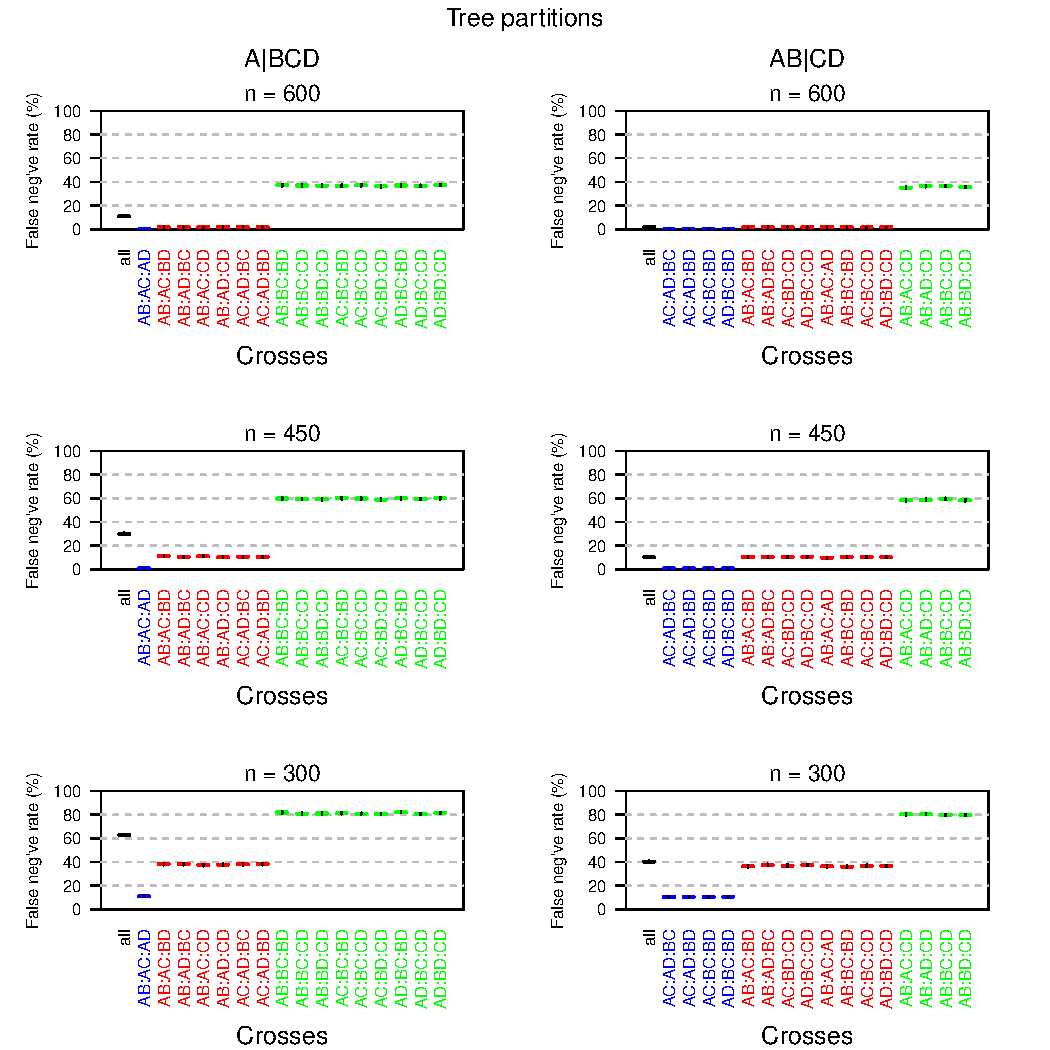
\includegraphics{SuppFigs/detailedns_treepart.pdf}}

\bigskip \noindent
Figure S16: Detailed results on the estimated false negative rate for individual
  choices of crosses, in the case of four taxa related as in Figure~1,
  with a total sample size of either 300 (bottom panels) 450 (middle
  panels) or 600 (top panels), and with the QTL being responsible
  for 10\% of the phenotypic variance in crosses in which it is
  segregating. Blue, red and green correspond to cases in which 3, 2,
  and 1 of the crosses are segregating the QTL, respectively.  The
  results are based on 10,000 simulation replicates, with analyses
  considering only the four possible partitions induced by the tree.
  The black vertical line segments indicate 95\% confidence intervals.


\newpage

\centerline{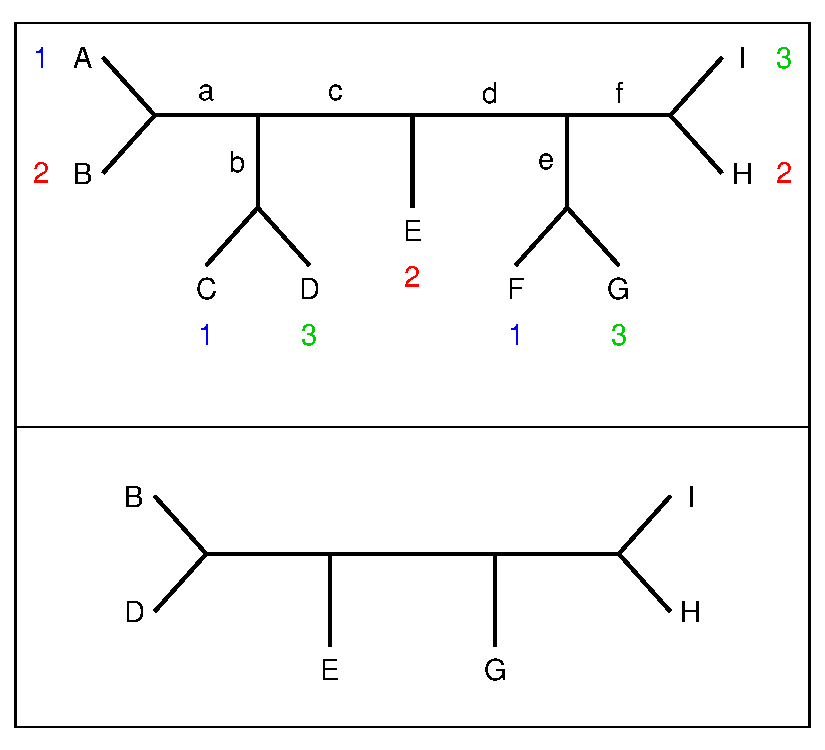
\includegraphics{SuppFigs/supp_tree_fig.pdf}}

\bigskip \noindent
Figure S17: Illustration of the construction of a minimal set of
crosses to distinguish the partitions induced by a tree.  In the upper
panel, the nine taxa (indicated with upper-case letters) are divided
into three groups (indicated with numbers) by the method
described in the Appendix.  Internal edges are indicated with
lower-case letters.  The lower panel contains the subtree of
six taxa defined by excluding the first group of three taxa (A, C, and F).
The method described in the Appendix identifies the set A$\times$C,
C$\times$F, B$\times$E, E$\times$H, D$\times$G, and G$\times$I as six
crosses sufficient to distinguish all 15 partitions induced by the tree.


\newpage

\noindent Table S1: Estimated 5\% genome-wide significance thresholds,
based on 10,000 simulation replicates, for a single intercross.  We
assumed an autosomal genome modeled after the mouse, with genetic
markers at a 10~cM spacing.

\bigskip
\bigskip

\renewcommand{\arraystretch}{1.8}
\begin{center}
\begin{tabular}{cc}
\hline
sample size    &   threshold \\ \hline
50    &  3.80 \\ 
75    &  3.72 \\
100   &  3.65 \\ \hline
\end{tabular}
\end{center}


\newpage

\noindent Table S2: Estimated 5\% genome-wide significance thresholds
for the maximum LOD score across partitions in the case of four taxa,
based on 10,000 simulation replicates.  We
assumed an autosomal genome modeled after the mouse, with genetic
markers at a 10~cM spacing.

\bigskip
\bigskip

\renewcommand{\arraystretch}{1.8}
\begin{center}
\begin{tabular}{cc cc c cc}
\hline
total             &\hspace*{5mm}& \multicolumn{2}{c}{All partitions} &\hspace*{5mm}& \multicolumn{2}{c}{Tree partitions} \\
 \cline{3-4} \cline{6-7}
sample size      && all crosses & minimal crosses  && all crosses &  minimal crosses \\ \hline
300              &&     4.56  &      4.48  &&     4.43   &      4.33 \\ 
450              &&     4.51  &      4.47  &&     4.36   &      4.33 \\
600              &&     4.49  &      4.44  &&     4.32   &      4.29 \\ \hline
\end{tabular}
\end{center}


\end{document}
